\subsection{Opgaver}
\begin{enumerate}
	\item En linje $l$ går gennem punkterne $(1,-6)$ og $(-2,3)$. Bestem både parameterfremstillingen og ligningen for $l$ samt linjens skæringspunkter med akserne.
	
	\item Linjen $l$ har ligning 
	\begin{align*}
	x+2y-6=0
	\end{align*}
	og linjen $m$ har parameterfremstilling
	\begin{align*}
	\begin{bmatrix}
	x\\y
	\end{bmatrix}= \begin{bmatrix}
	1\\1
	\end{bmatrix}+t \begin{bmatrix}
	2\\-1
	\end{bmatrix}
	\end{align*}
	hvor $t\in \R$. Gør rede for at $l$ og $m$ er parallelle.
	
	\item Bestem skæringspunkterne mellem cirklen $x^2+y^2=2$ og linjen med parameterfremstilling
	\begin{align*}
	\begin{bmatrix}
	x\\y
	\end{bmatrix}= \begin{bmatrix}
	3\\-3
	\end{bmatrix}+t \begin{bmatrix}
	1\\-1
	\end{bmatrix}.
	\end{align*}
	
	\item Bestem ligningen for linjen gennem punkterne $(-2,1)$ og $(1,-1)$. Hvordan ligger denne linje i forhold til linjen med parameterfremstilling
	\begin{align*}
	\begin{bmatrix}
	x\\y
	\end{bmatrix}= \begin{bmatrix}
	7\\-5
	\end{bmatrix}+t \begin{bmatrix}
	9\\-6
	\end{bmatrix}.
	\end{align*}
	
	
	
	
	\item Bestem parameterfremstillingen for linjen gennem punkterne $(-2,0)$ og $(5,5)$. Hvordan ligger denne linje i forhold til linjen med parameterfremstilling
	\begin{align*}
	-10x+14y=21
	\end{align*}
	
		
	\item Bestem parameterfremstillingen for linjen gennem punkterne  $(-6,-2)$ og $(8,8)$. Hvordan ligger denne linje i forhold til linjen med parameterfremstilling
	\begin{align*}
	3x+2y=9
	\end{align*}
	
	
	\item Bestem parameterfremstillingen for linjen det går gennem skæringspunkterne til de to cirkler 
	\begin{align*}
	(x-1)^2+(y-1)^2=1,&& (x+1)^2+(y+1)^2=5.
	\end{align*}
	
			\item\label{it:2dvec14} I Figur~\ref{fig:2dvec14} er linjerne $-x+y=1$ og $(2+\sqrt{3})x+y=3$ samt vinklen $\theta$ indtegnet. Bestem vinklen $\theta$. (Hint: Bestem koordinater til vektorer som ligger parallelt med de to linjer og bestem vinklen mellem dem. Det kan også være nødvendigt at anvende Opgave~\ref{it:root1})
	
	\begin{figure}
		\centering
		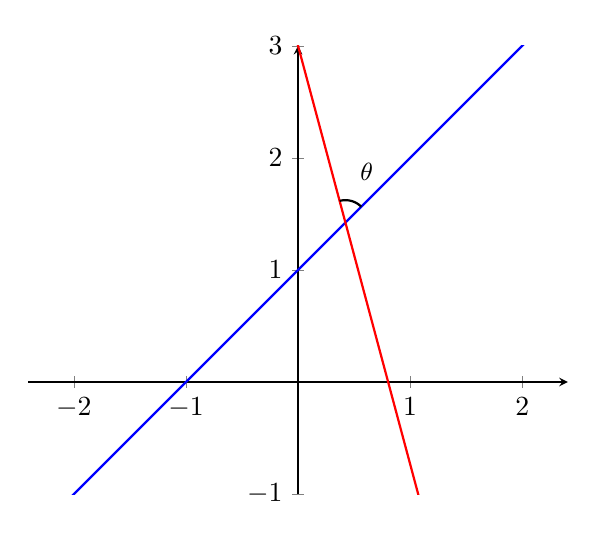
\begin{tikzpicture}
		\begin{axis}[xmin=-1,xmax=1,ymin=-1,ymax=3,axis x line=center,
		axis y line=center, axis equal]
		\addplot[thick,blue] {x+1};
		\addplot[thick,red] {-(2+sqrt(3))*x+3};
		\addplot[domain=pi/4:7*pi/12,thick,samples=100] ({2/(sqrt(3)+3)+0.2*cos(deg(x))},{(5+sqrt(3))/(sqrt(3)+3)+0.2*sin(deg(x))}) node[label=above right:\small$\theta$,pos=1] {};
		\end{axis}
		\end{tikzpicture}
		\caption{Opgave~\ref{it:2dvec14}}
		\label{fig:2dvec14}
	\end{figure}
	
	
	\item\label{it:2dvec15} I denne opgave vil vi projicere vektorer. Lad $\vec{u}$ og $\vec{v}$ være vektorer. Projektionen af $\vec{u}$ på $\vec{v}$ er en vektor $\vec{w}$ der har samme retning som $\vec{w}$ og så at afstanden fra $\vec{u}$ til $\vec{v}$ er mindst mulig. linjestykket fra $\vec{u}$ til $\vec{w}$ må derfor være vinkelret på $\vec{w}$.
	
	\begin{enumerate}
		\item På Figur~\ref{fig:2dvec15} ses en skitse af vektorerne $\vec{u}$, $\vec{v}$ og $\vec{w}$. Argumenter vha. trekanten afgrænset af $\vec{u}$, $\vec{w}$ og $\vec{u}-\vec{w}$ at 
		\begin{align*}
		\cos(\theta)=\frac{\norm{\vec{w}}}{\norm{\vec{u}}}.
		\end{align*}
		
		\item Brug formlen for vinklen mellem $\vec{u}$ og $\vec{v}$ til at konkludere at 
		\begin{align}\label{eq:2dvec11}
		\norm{\vec{w}} =\frac{\vec{u}\cdot \vec{v}}{\norm{\vec{v}}}.
		\end{align}
		
		\item Da $\vec{v}$ og $\vec{w}$ har samme retning gælder at
		\begin{align*}
		\frac{\vec{w}}{\norm{\vec{w}}}=\frac{\vec{v}}{\norm{\vec{v}}}.
		\end{align*}
		Brug dette sammen med~\eqref{eq:2dvec11} til at vise at projektionen $\vec{w}$ af $\vec{u}$ på $\vec{v}$ er givet ved
		\begin{align*}
		\vec{w}=\frac{\vec{u}\c \vec{v}}{\norm{\vec{v}}^2}\vec{v}
		\end{align*}
		
		
	\end{enumerate}
	\begin{figure}
		\centering
		\begin{tikzpicture}
		\begin{axis}[xmin=-0.1,xmax=4,ymin=-0.1,ymax=5,axis x line=center,
		axis y line=center, axis equal]
		\addplot[domain=0:1,thick,blue,->] {x} node[pos=0.5,below] {$\vec{v}$};
		\addplot[domain=0:(1+sqrt(3)),thick,gray,dashed,->] {x} node[pos=0.8,below] {$\vec{w}$};
		\addplot[domain=0:2,thick,red,->] {sqrt(3)*x} node[pos=0.5,above,left] {$\vec{u}$};
		\addplot[domain=2:(1+sqrt(3)),dotted,gray,thick,<-] {-1*x+2+2*sqrt(3))} node[pos=0.5,above,right] {$\vec{u}-\vec{w}$};
		\addplot[domain=pi/4:pi/3,thick,samples=100] ({0.4*cos(deg(x))},{0.4*sin(deg(x))}) node[label=above right:\small$\theta$,pos=1] {};
		\end{axis}
		\end{tikzpicture}
		\caption{Opgave~\ref{it:2dvec15}}
		\label{fig:2dvec15}
	\end{figure}
	
	\item Lad 
	\begin{align*}
	\vec{u}=\begin{bmatrix}
	1\\2
	\end{bmatrix}, \quad \textup{og} \quad \vec{v}_1=\begin{bmatrix}
	6\\2
	\end{bmatrix},\quad \textup{og} \quad \vec{v}_2=\begin{bmatrix}
	-3\\-6
	\end{bmatrix}\quad \textup{og} \quad \vec{v}_3=\begin{bmatrix}
	-4\\2
	\end{bmatrix}.
	\end{align*}
	Beregn 
	\begin{enumerate}
		\item projektionen af $\vec{u}$ på $\vec{v}_1$.
		\item projektionen af $\vec{u}$ på $\vec{v}_2$.
		\item projektionen af $\vec{u}$ på $\vec{v}_3$.
	\end{enumerate}

%	\item Bestem afstanden fra punktet $P=(2,3)$ til linjen $l$ givet ved $3x+2y=0$. Bestem efterfølgende afstanden fra $P$ til linjen $m$ givet ved $3x+2y=1$.
\end{enumerate}